
\documentclass[a4paper,10pt]{article}
\usepackage[margin=2cm]{geometry}

%%% Language and encoding %%%
\usepackage[utf8]{inputenc}
\usepackage[T1]{fontenc}
%%% Mathematical symbols and notations %%%
\usepackage{amsthm, amsmath, mathrsfs, amssymb}
\usepackage{textcomp}
\usepackage{algorithm}
\usepackage{algorithmic}

%%% Figures %%%
\usepackage{caption, subcaption}
\usepackage{tikz}
\usepackage{tkz-graph}
\usetikzlibrary{shapes, shapes.gates.logic.US, trees, positioning, arrows, decorations.pathreplacing, plotmarks, backgrounds,shapes}
%%% Other packages %%%
\usepackage[affil-it]{authblk}
\usepackage{multirow}
\usepackage{xcolor}
\definecolor{bleuclairimtatlantique}{RGB}{0,184,222}
\definecolor{noirimtatlantique}{RGB}{60, 60, 60}
\definecolor{blancimtatlantique}{RGB}{255, 255, 255}
\definecolor{bleufonceimtatlantique}{RGB}{12, 35, 64}
\definecolor{vertimtatlantique}{RGB}{164, 210, 51}
\definecolor{grisimtatlantique}{RGB}{230, 230, 230}
\definecolor{ocre}{RGB}{250,82,20}
\usepackage{url}
\usepackage{hyperref}
\usepackage{verbatim}
\usepackage{varwidth}
%% Define the figures path
\newcommand{\inputfig}[1]{\input{figures/#1}}
\graphicspath{{figures/}}

%\usepackage{empheq}
\usepackage[framemethod=tikz]{mdframed}

%%%%% Definition of commands %%%%%
\newcommand{\loc}{\mathcal{L}}
\newcommand{\cu}{\mathcal{C}}
\newcommand{\su}{\mathcal{S}}
\newcommand{\ro}{\mathcal{R}}

%%%%% Definitions for tikz %%%%%
% Definition of styles for diagrams :
\tikzset{%
    % Symbols for block diagrams
    block/.style    = {draw, thick, rectangle, minimum height = 3em,
    minimum width = 3em},
    sum/.style      = {draw, circle, node distance = 2cm}, % Adder
    input/.style    = {coordinate}, % Input
    output/.style   = {coordinate}, % Output
    % Gates and symbols style for the fault trees
    and/.style={and gate US,thick,draw,fill=red!20,rotate=90,
    anchor=east,xshift=-1mm},
    or/.style={or gate US,thick,draw,fill=blue!20,rotate=90,
    anchor=east,xshift=-1mm},
    be/.style={circle,thick,draw,fill=green!20,anchor=north,
    minimum width=0.7cm},
    tr/.style={buffer gate US,thick,draw,fill=purple!40,rotate=90,
    anchor=east,minimum width=0.8cm},
    % Label style
    label distance=3mm,
    every label/.style={blue},
    % Event style
    event/.style={rectangle,thick,draw,fill=yellow!10,text width=2cm,
    text centered,font=\sffamily,anchor=north},
    % Children and edges style
    edge from parent/.style={very thick,draw=black!70},
    edge from parent path={(\tikzparentnode.south) -- ++(0,-1.05cm)
    -| (\tikzchildnode.north)},
    level 1/.style={sibling distance=7cm,level distance=1.4cm,
    growth parent anchor=south,nodes=event},
    level 2/.style={sibling distance=7cm},
    level 3/.style={sibling distance=6cm},
    level 4/.style={sibling distance=3cm},
    %%  For compatability with PGF CVS add the absolute option:
    absolute
}

\tikzstyle{client}=[regular polygon,regular polygon sides=3,draw,fill=blue!50,fill opacity=1,scale=0.4]
\tikzstyle{ptf}=[draw,circle,fill=red!50,fill opacity=1,scale=0.8]
\tikzstyle{cdc}=[regular polygon, regular polygon sides=3,draw,fill=yellow!70,fill opacity=1,scale=1.2]

\tikzstyle{legend}=[scale=0.7,right,text justified]
\tikzstyle{shipment}=[->,>=stealth',blue]
\tikzstyle{ftlarc}=[->,>=stealth',very thick,red]
\tikzstyle{vertexD}	=[circle,draw=black!80,fill=purple!70,minimum size=7pt,inner sep=0pt]
\tikzstyle{vertex0}	=[circle,draw=black!80,fill=purple!20,minimum size=7pt,inner sep=0pt]
\tikzstyle{j0}			=[circle, draw=black,fill=purple,minimum size=13pt,inner sep=0pt, scale=1]
\tikzstyle{farm}		=[circle, draw=black,fill=blue!80,minimum size=4pt,inner sep=0pt, scale=1]

\tikzstyle{com2}		= [minimum size=0pt,inner sep=0pt, scale=1]
\tikzstyle{edgetr} 	= [draw,thick,->,purple]
\tikzstyle{edge1} 	= [draw,dotted,-,blue, thick]



\title{Location Inventory Routing Problem: new formulation and sampling heuristic}
	
\author{Guillaume Massonnet$^{1,2}$, Olivier P\'eton$^{1,2}$}
	
\date{$^1$ IMT Atlantique\\ 
	$^2$ LS2N UMR CNRS 6004 (Laboratoire des Sciences du Numérique de Nantes), \\ 4 rue Alfred Kastler, F-44307 Nantes Cedex, France}
	%\cortext[cor]{Corresponding author. name address}
	
\begin{document}
	
\maketitle

\begin{abstract}
	blablabla
	
	
\textbf{Keywords:}	facility location, inventory management, routing, sampling heuristics, supply chain
	
\end{abstract}


\OP{Choix de vocabulaire: level }
\OP{client ou customer ? }



\modulolinenumbers[5]
\linenumbers
\begin{linenumbers}


\section{Introduction}


Logistics and supply chain management decisions in industry are traditionally divided into 
\textit{strategic decisions}, which concern the definition and sizing of long-term resources, 
\textit{tactical decisions}, which concern the use of resources over a period of a few months and 
\textit{operational decisions}, which concern daily or weekly operations. 
In a distribution network, examples of strategic decision are the location of production facilities and distribution centers (DC), the allocation of customer to distribution centers. 
Inventory and fleet management fall into the category of tactical decisions,
 whereas vehicle routing belong to operational decisions. 

In some companies, logistics decisions can be taken independently of each others. 
In this case, strategic decisions are typically taken or revised every year, then tactical decisions are taken every month assuming known strategic choices, and operational decision are taken every day or week assuming known tactical decisions. 
However, in many companies and activities, strategic, tactical and operational decisions are interrelated. 
For example, the choice of a location for a truck depot highly influences the quality of routing, so that finding the best location without considering routing aspects would probably lead to a bad location decision.  Integrated Location Routing Problems (LRP) have been studied for several decades. Recent surveys include \cite{ProdhonPrins2014}, \cite{DrexlSchneider2015} and \cite{Schneider2017}.  
  

Another example in the inventory routing problem (IRP). 
The IRP considers one supplier running a fleet of vehicles and a set of customers who consume a good on a multi-period time horizon. The objective of the IRP is to jointly optimize the delivery schedule of customers, the quantities delivered, and the delivery routes to be covered in each period, while minimizing the sum of routing costs and storage costs. The popularity of the IRP has grown with the development of the Vendor Managed Inventory (VMI) system, in which the supplier monitors the inventory and decides the replenishment policy of each retailer \cite{Archetti2007}. 
The IRP has been studied for more than 30 years \cite{Coelho2014}. Prior surveys had been published by \cite{Campbell98}, \cite{MoinSalhi2007}. Interested reader may also read the tutorial by \cite{Bertazzi2012}. 
Very few models consider the inventory routing problem within a two-echelon or multi-echelon network	\cite{GuimaraesCoelho2019}

Traditional applications of the IRP have been listed in the survey \cite{Coelho2014}. They mainly concern the distribution of commodities, raw materials or fast moving consumer goods. These activities rely on a stable supply chain network. 
In industrial applications the set of customers is quite stable and the starting points of all defined for a long duration.
For example, distribution of fuel always starts from the same fuel depots, which capacity and location cannot be easily modified. 

As pointed by \cite{Melo2009}, facility location is frequently combined with inventory decisions. 
The Inventory Location Problem (ILP) aims at determining the optimal number of distribution centers,  their locations,  the retailers assigned to each distribution center  and the optimal ordering policy at the distribution centers.  Reviews on inventory location problems have been proposed by \cite{kaviani_location-inventory_2009} 
and \cite{farahani_location-inventory_2015}. 

In this paper we consider the integrated optimization problem of jointly optimize facility location, inventory management and vehicle routing. This optimization problem, called the Location Inventory Routing Problem (LIRP), recently appeared in the scientific literature \cite{AhmadiJavid2010}. It is relevant when considering an IRP on a supply chain which is not stabilized yet or must be frequently revised (e.g., delivery of e-commerce goods or services to a set of customers that changes over time). We consider a three-layer supply chain consisting of one production facility, several intermediate depots called Distribution Centers (DC) and a larger set of customers. Product are first carried from the production facility to DCs, and then from DCs to customers. The decision variables concern the location of DCs, the allocation of customers to DC as well as the IRP routing and inventory decisions. 

The outline of this paper are the following. 
In section \ref{sec:lit}, we review the scientific literature dedicated to the LIRP. 
In section \ref{sec:model}, we propose a new mathematical formulation of the LIRP and show that this formulation is general enough to cover several types of supply chain networks. 
In section \ref{sec:algo}, we propose a Route Sampling Heuristic (RSH) algorithm for the LIRP. 
In section \ref{sec:expe}, we introduce new LIRP instances and report numerical experiments that show the performance of our algorithm.




\section{Review of the literature} \label{sec:lit}

The location inventory routing problem LIRP has been attracting much research effort in the very recent years, but preliminary works have appeared several decades ago.  
In this section, we review the main publications related to the LIRP.
Section \ref{sec:almost} summarizes the preliminary works that led to a formal definition of the LIRP. 
Next sections described the modeling of the main LIRP components: location and supply chain design (section \ref{sec:l}), 
routing (\ref{sec:r} and inventory policies (\ref{sec:i}). 

\subsection{Preliminary works related to the LIRP}
\label{sec:almost}

 The idea of integrating location, inventory and routing decisions in mathematical models is not new, but most models have been considered intractable until the recent progress of mathematical programming solvers and heuristic solution methods. 
In 1988, \cite{PerSir88} pointed the necessary interdependence between location, inventory and routing decisions. 
The authors proposed an integrated model combining location and inventory decisions, but only direct shipments were considered and no computational experiments were presented. 
This model has been extended by \cite{AmbScu05} to a multi-level problem with distribution routes visiting several customers. The authors also propose a dynamic models (with multiple periods). Computational experiments show the practical difficulty of solving static models (with one time period). 


Several LIRP related papers considered the three main decisions in a hierarchical way, or priority is given to one or two decisions. 
In \cite{LiuLee03} and \cite{LiuLin05}, inventory management decisions are taken independently from routing and location. 
\cite{Shen07} explicitly model facility location and allocation decisions but use approximated routing costs instead of formal routing costs. 
\cite{MetZab10} propose a two-stage stochastic programming approach for a medical supply
storage and distribution problem.
At the first stage, storage locations and the optimal inventory policy are determined. 
At the second stage, a recourse routing plan is optimized for each disaster scenario. 
Routing decision are decoupled from location and inventory decisions. 
Hence, all these references cannot be \textit{stricto sensu} considered as LIRP models. 

\subsection{Supply chain design}
\label{sec:l} 

As an integrated optimization problem, the LIRP usually arises in complex logistics networks with several level of facilities. 
Depending on the volume of the shipments, transport can be organized in full truckload (FTL) or less than truckload (LTL) legs. 
In FTL transport, shipments are sent directly from their origin to their destination. In LTL transport, routes have one origin and several delivery points. The roads are therefore multi-clients. The presence of a ``routing'' component in the LIRP assumes the existence of routes visiting multiple sites, at least in one part of the supply chain.
The vast majority of LIRP articles deal with three-level networks such as that illustrated in Figure \ref{fig:directloop}. 
Direct routes are performed between a production facility (large red circle) delivers a set of DCs (small red circles). A second echelon includes routes visiting several end customers (blue circles).

\begin{figure}[htbp]
	\centering
	\inputfig{model1}
	\caption{LIRP model with direct+route supply chain design}
		\label{fig:directloop}
	\end{figure}

Several papers deviate from this main scheme.  \cite{Zhang2014} consider only 2 levels: a set of candidate depots and customers. Routes start at a depot and visit several customers ; no inventory decision is made at depots. 

\cite{AmbScu05} and \cite{Tavana2018} extend the main logistics scheme to a 4 level network. Shipments are direct in the upper echelon whereas LTL routes are performed in the two lower echelons. 
\cite{Eskandari2018} study a blood supply chain with 4 level. They consider direct shipment between the first three levels and multi-point routes for the final delivery. 
\cite{Bashiri2018} consider a network with multi-point routes at the first echelon and direct deliveries at the second echelon. 
Finally, \cite{Riquelme2016} introduce the location arc routing problem with inventory constraints. 

Moreover, only a few papers (\cite{LiuChenLiLiu2015}, \cite{Deng2016}, \cite{Zhalechian2016} and \cite{LiGuoWangFu2013} 
consider a closed-loop supply chain. 


\subsection{Route formulation}
\label{sec:r}

A large majority of the LIRP mathematical models uses an arc-based representation of the routes. 
However, in many applications, the number of customer visited within a route is limited by a number of practical constraints (time constraints, stopover costs, detour constraints). \cite{MaDav05} propose a distribution chain design  minimizing location fixed costs, inventory costs and transportation costs. They observe that vehicles can only serve one site in their journey, and thus, do not model a full LIRP model. 

\cite{Guerrero2013} propose a route-based model with an exponential number of routes. A relaxation of the model is decomposed into an inventory location problem and a routing problem which is solved by column generation. 
The model in \cite{Lehrlaly2016} is based on all feasible routes with no more than three customers. 
Route based models are also used in \cite{LiGuoWangFu2013}, \cite{LiuChenLiLiu2015},  \cite{Deng2016} and \cite{hiassat_genetic_2017} 
but these papers do not detail routes generation.

\subsection{Inventory policies}
\label{sec:i}

As far as inventory management is concerned, the literature can be classified in two main families: 
some papers consider a continuous time inventory policy whereas others consider discretized time periods. 
In the first category, demand is considered either constant (see e.g. \cite{AhmSed2012}, \cite{Deng2016})
or subject to a given distribution such as the normal distribution (see e.g. \cite{Zhalechian2016}, \cite{Saragih2018}) or 
the Poisson distribution (see e.g. \cite{Asadi2018}, \cite{HabibiAS2018}). 
\cite{AhmadiJavid2010}, \cite{AhmSed2012}, \cite{Seyedhosseini2014}, \cite{LiuChenLiLiu2015}, \cite{Tang2016}, \cite{Deng2016} and  \cite{Saragih2018} apply the $(r,Q)$ inventory review policy whereas \cite{Dehghani2017}, \cite{HabibiAS2018} and \cite{Asadi2018} apply the $(S-1,S)$ policy. \cite{Yuchi2016} use the Wilson formula. 
Note that in  most of these works, the objective function incorporates the average value of inventory or their standard deviation, which yields non linearity. 
Thus, only small instances can be solved by MINLP solvers, or general purpose heuristics and metaheuristics are used. 

Note that all papers presenting continuous time inventory policy consider logistics network with three layers. 
Direct shipments are performed from layer 1 to layer 2 and routes between a facility at layer 2 and several client at layer 3. 
\cite{LiuChenLiLiu2015} and \cite{Deng2016} propose route based models ; all other references propose arc based models. 


In this paper, we use discretized time periods and all demands and material flow values within one period are aggregated. This leads to inventory management policies that can be modeled by lot sizing optimization problems. 
All papers use multiple period formulation. Note that \cite{AmbScu05} formulated a mathematical model with multiple periods but provide solutions with a single period only. 
Most LIRP references consider models in which all data are deterministic but variable (see e.g. \cite{Guerrero2013}, \cite{Zhang2014}, \cite{Ghorbani2016}). 
\cite{Vahdani2018} consider stochastic storage capacity. 
\cite{Rayat2017} explicitly model stochastic demand and propose an MINLP bi-objective model with multiple periods and multiple products. The model is solved with an epsilon constraint and several multi-objective metaheuristics. 
Uncertainty can also be incorporated through various modeling techniques. 
\cite{ChenChenSunLiu2014, TavakkoliIFAC2016, Eskandari2018} model fuzzy demand and parameters ; \cite{Bashiri2018} define demand scenarios ; 
\cite{Zhalechian2016} and \cite{Rafie-Majd2018} consider demands following a normal distribution and combine discretized time modeling with a $(R,Q)$ replenishment policy.  

Table \ref{tab2} presents the main features of LIRP models with time discretization. 

\begin{table}[htbp]
	\centering
	\scriptsize
	\begin{tabular}{lccclc}
		\toprule
		Reference &  Route & Network    & Flow &  \multicolumn{1}{c}{Uncertain}  & Linear  \\
				  & model & layers	   & 	   &   \multicolumn{1}{c}{data}       &                      \\
		\midrule
\cite{AmbScu05}				&	arc		&	4 	&	direct+loop+loop	&		&	\checkmark		\\
\cite{Zhang2014}			&	arc  	&	2 	&	loop				&		&	\checkmark	\\
\cite{Guerrero2013}			&	route	&	3 	&	direct+loop			&		&	\checkmark	\\
\cite{Nekooghadirli2014}	&   arc 	&	3   &   direct+loop			& 	\checkmark &  	\\	
\cite{TavakkoliIFAC2016}	&	arc		&	3 	&	direct+loop			&	\checkmark (fuzzy) 	&	\checkmark	\\
\cite{Ghorbani2016}			&	arc		&	3 	&	direct+loop			&		&	\checkmark \\
\cite{Lehrlaly2016}			&	route	&	3 	&	direct+loop			&		&	\checkmark		\\
\cite{Rayat2017}			&	arc		&	3 	&	direct+loop			&	\checkmark	&			\\
\cite{Zhalechian2016}		&	arc		&	3	& 	direct+loop			&	\checkmark	& 	\\	
\cite{Hiassat2017}			&	route	&	3 	&	direct+loop			&		&	\checkmark		\\
\cite{Riquelme2016}			&	arc		&	2 	&	general graph		&		&	\checkmark	\\
\cite{Tavana2018} 			&	arc		&	4 	&	direct+loop+loop 	&		&	\checkmark		\\
\cite{Vahdani2018}			&	arc		&	3 	&	direct+loop			&	\checkmark			&	\checkmark	\\
\cite{Eskandari2018}		&	arc		&	4 	&	direct+direct+route	&	\checkmark (fuzzy)	&	\checkmark		\\
\cite{Bashiri2018}			&	arc		&	3 	&	loop+direct			&	\checkmark (scenario)	&	\checkmark	\\
\cite{Rafie-Majd2018}		& 	arc		&	3 	&  	direct + loop 		&  \checkmark 			&  \\	
\textit{This paper}			& route		& any	&   flexible			& 						& \checkmark \\
		\bottomrule
	\end{tabular}
	\caption{LIRP papers using time discretization}
	\label{tab2}
\end{table}




\subsection{Contribution of this paper}

This paper brings contribution in the LIRP literature in three ways. 
First, we propose new route-based mathematical model for a multi-level logistics network with both FTL and LTL routes. 
Without loss of generality, we describe a network with one production facility, multiple levels of candidate distribution centers and a larger set of customers at the last level. 
Second, we propose a sampling solution method based on the decomposition of large instances in several smaller instances that are tractable by an MILP solver. 
Finally, we introduce new instances for the LIRP and present computational experiments that show the relevance of our approach. 

\OP{Vérifier l'argumentation FTL, LTL}

%-------------------------------------------------------

\section{Mathematical model}

\label{sec:model}

\subsection{Problem settings and notations}\label{subsection:settings}


In this section, we introduce a new mixed integer linear programming formulation for the LIRP, 
that covers a broad spectrum of potential applications and distribution networks. 
In particular, the model includes the possibility of dealing with multiple levels of DCs and FTL or LTL distribution (see, e.g. \cite{AmbScu05}). 

We consider a distribution network composed of one production center, several layers of distribution centers and a terminal layer of customers. Let us call $\loc$ the set of all facility locations (DCs and customers) in the distribution network. 
We assume that $\loc$ is decomposed into levels and we denote by $\loc_k$ the set of facility locations at level $k$. 
A DC lies on level 1 if it is delivered by the production facility only. 
It lies at level $k$ if it is delivered by at least one DC from level $k-1$. 
Let $L$ be the number of levels in the networks. By definition, the set $\cu$ of customers corresponds to $\loc_L$.
Moreover, $\loc=\bigcup\limits_{k=1}^L \loc_k$.
%
Selecting a DC incurs a fixed opening cost $f_j$ for each DC. 
This cost is paid once at the beginning of the planning horizon. 
Note that the choice of selected DCs cannot be modified during the whole time horizon. 
%
Customers demand is assumed deterministic on a given time horizon $T$, typically a few weeks. The demand of customer $i \in \cu$ at time period $t\in T$ is denoted by $d^t_i$.
%
Storage of goods at DCs and customers is authorized, 
but incurs a holding cost $h^t_i$ for every good stored at facility $i \in \loc$ at period $t \in T$.
The initial inventory at facility $i \in \loc$ is denoted by $I_i^0$. 
We assume that inventory level at facility $i \in \loc$ cannot excess maximal value $I_i^{\max}$. 

Our proposed formulation is based on a set of existing routes in the logistics network. 
This set $\ro$ is potentially large but enumerable. 
Similarly to the set of facilities, the set of routes can be decomposed in levels: $\ro = \bigcup\limits_{k=1}^{L} \ro_k$. 
All routes $r \in \ro_k$ start from a facility (production facility or DC) at level $k-1$ and deliver facilities at level $k$. 
For each route $r \in \ro$, the list of facilities visited is given by an indicator vector. 
For the sake of clarity, we define two indicators: 
$\beta_{jr}$ is equal to 1 if $r$ starts from DC $j \in \loc \setminus C$, and 0 otherwise;
$\alpha_{ir}$ is equal to 1 if route $r \in \ro_{L}$ visits facility $i \in \loc$, and 0 otherwise.
%

Each route 	$r\in \ro$ has a deterministic cost $c_r$ that consists of a (possibly zero) fixed ordering cost, 
a routing cost roughly proportional to the route length and stopover costs for each facility visited.  
Finally, each route level is operated by a homogeneous fleet of vehicles. 
Let $\nu_k$ the number of vehicles available at level $k$ and $Q_k$ their capacity. 
%



The proposed MILP formulation is based on the following sets of binary variables: 
$$	y_j  = \left\{
\begin{array}{ll}
1 & \mbox{if distribution center } j \mbox{ is selected }  \\
0 & \mbox{otherwise.}
\end{array}
\right.
$$
$$	z_{rt}  = \left\{
\begin{array}{ll}
1 & \mbox{if route } r \in R \mbox{ is selected in period } t \in T \\
0 & \mbox{otherwise.}
\end{array}
\right.
$$

Moreover, continuous variables $x_{irt} \geq 0$ and $I_{it} \geq 0$  
determine the quantities delivered by route $r \in \ro$ to facility $i \in \loc$ in period $t\in T$
and the inventory at facility $i \in \loc_{k}$ in period $t \in T$, respectively. 
Tables \ref{tab:set}--\ref{tab:var} summarize the mathematical notations that will be used throughout the paper.

\begin{table}[htbp]
	\centering
	\begin{tabular}{ll}
		\toprule
		$T$ & Set of time periods. $T = 1,\dots,|T|$\\
		$L$ & Number of levels in the distribution network\\
		$\loc_k$ & Set of locations at level $k=1, \ldots,L$ \\
		$\cu=\loc_L$ & Set of customers \\ 
		$\loc=\cup_{k=1}^L \loc_k$ & Set of all locations in the distribution network\\
		$\ro_k$ & Set of routes at level $k$\\
		$\ro = \cup_{k=1}^{L} \ro_k$ & Set of all routes in the distribution network\\
		\bottomrule
	\end{tabular}
	\caption{Data sets and parameters}
	\label{tab:set}
\end{table}       


\begin{table}[htbp]
	\centering
	\begin{tabular}{ll}
		\toprule
		$f_j$ & Fixed cost of opening distribution center $j\in\loc \setminus \cu$\\ 
		$d_{it}$ & Demand of customer $i\in\cu$ in period $t \in T$\\
		$h_{it}$ & Unitary holding cost at facility $i\in\loc$ in period $t \in T$\\
		$I_{i0}$ & Initial inventory at facility $i\in \loc$\\
		$I_i^{\max}$ & Maximum inventory at location $i\in\loc$\\
		$c_r$ & Cost of route $r\in \ro$\\
		$\alpha_{ir}$ & Indicator that route $r$ delivers facility $i \in \loc$\\
		$\beta_{jr}$ & Indicator that route $r$ starts from DC $j \in \loc \setminus \cu$\\
		$Q_k$ & Capacity of vehicles delivering locations at level $k$\\ 
		$\nu_k$ & Fleet size for vehicles delivering locations of level $k$\\ 
		\bottomrule
	\end{tabular}
	\caption{Data}
	\label{tab:data}
\end{table}       


	\begin{table}[htbp]
	\centering
	\begin{tabular}{ll}
		\toprule
		\multicolumn{2}{l}{\textit{Binary Variables}}\\
		$y_{j}$ & $=1$ if distribution center $j \in \loc \backslash \cu$ is selected \\
		$z_{rt}$ & $=1$ if route $r \in \ro$  is selected in period $t \in T$\\
		\midrule
		\multicolumn{2}{l}{\textit{Continuous variables}}\\
		$x_{irt}$ & Quantity delivered by route $r \in \ro$ to location $i\in \loc$ in period $t\in T$\\
		$I_{it}$ &  Inventory at location $i \in \loc$ in period $t \in T$\\
		\bottomrule
	\end{tabular}
	\caption{Variables}
	\label{tab:var}
\end{table}    


\subsection{Mathematical  formulation}\label{subsection:MIP}

The objective function to be minimized can be stated as follows: 
 
\begin{equation} \label{objfunct}
    \text{minimize} \sum_{j\in \loc \setminus \cu} f_{j} y_{j} +\sum_{t\in T} \left( \sum_{r\in \ro} c_r z_{rt} + \sum_{i\in \loc} h_{it} I_{it}\right)
    \end{equation} 
    
    The first term in equation (\ref{objfunct}) represents the sum of fixed opening costs for all DCs selected. 
    The second term is the sum of all routing costs and inventory costs during the time horizon considered. 
    
  The LIRP is subject to the following constraints:
    
    \begin{alignat}{3}
&&\sum_{r\in \ro_L} \alpha_{ir} z_{rt} &\leq 1 						&\forall i&\in \cu, t \in T  					\label{const:singleroutecustomers}\\
&&\sum_{r\in \ro_k} \alpha_{jr} z_{rt} &\leq y_j 					&\forall k&=1,\ldots,L-1, j\in \loc_k, t \in T  \label{const:singleroutedc}\\
&&z_{rt} 					&\leq \sum_{j\in\loc_{k}}\beta_{jr}y_j 	&\forall k&=1,\ldots,L-1,r\in \ro_{k+1}, t \in T \label{const:startfromopendepots}\\
&&\sum_{r\in \ro_k} z_{rt} &\leq 	\nu_k							&\forall k&=1,\ldots,L, t \in T  				\label{const:fleetcapa}\\
&&\sum_{i\in \loc_k} x_{irt}   		&\leq Q_k z_{rt} 			&\forall k&=1,\ldots,L,  r\in \ro_k, t \in T 	\label{const:deliveryUB}\\
&&x_{jrt}   		&\leq \alpha_{jr} Q_k  						&\forall k&=1,\ldots,L,  r\in \ro_k, j \in \loc_k, t \in T	\label{const:deliveryConstLoc}\\
&&I_{jt} - I_{j,t-1} &= \sum_{r\in\ro_k} x_{jrt} 	- \sum_{r'\in \ro_{k+1}}\left(\beta_{jr'} \sum_{i\in \loc_{k+1}}x_{ir't}\right)\quad 						&\forall k&=1,\ldots,L-1, j\in \loc_k, t \in T 				\label{const:invflowdepots}\\
&&I_{it} - I_{i,t-1} &= \sum_{r\in \ro_L} x_{irt} - d_{it} 			&\forall i&\in \cu,  t \in T					\label{const:invflowcustomers}\\
&&I_{jt}	&\leq I_j^{\max} y_j  									&\forall k&=1,\ldots,L-1,  j\in \loc_k, t \in T \label{const:invdepotUB}\\	
&&I_{it} 	&\leq \min\left(I_i^{\max}, \sum_{t' > t}d_{it'}\right)	&\forall i&\in \cu,  t \in T					\label{const:invcustUB}\\
&&x_{irt}			&\geq 0 										&\forall k&=1,\ldots,L,  i\in \loc_k,  r\in \ro_k,\forall t \in T	\label{const:upos}	\\
&&I_{it}			&\geq 0 										&\forall i &\in \loc,  t \in T					\label{const:invCpos}	\\
&&y_{j}				& \in \{0,1\} 								&\forall j&\in \loc\setminus\cu						\label{const:ybool}\\	
&&z_{rt}			&\in \{0,1\} 									&\forall r&\in \ro,  t \in T.					\label{const:zbool}
\end{alignat}


Single delivery constraints~\eqref{const:singleroutecustomers} state that, at any period, each customer is delivered by at most one route. 
%
Constraints ~\eqref{const:singleroutedc} express the same idea for DCs: at any period, DCs are served by at most one route serving the corresponding level. Moreover, this constraint prevents from delivering non selected DCs. 
%
Constraint~\eqref{const:startfromopendepots} ensures that a route at level $k+1$ can start only from a DC selected at level $k$ (Note that by definition $\sum_{j\in\loc_{k}} \beta_{jr} \leq 1$).
%
Constraints~\eqref{const:fleetcapa} states that the number of routes used to serve the locations of a given level $k$ in period $t$ does not exceed the number of vehicles allocated to that level. 
%
Constraints~\eqref{const:deliveryUB} ensure that the sum of the quantities delivered through a route $r\in\ro_k$ in period $t$ is compatible with the vehicles capacity. 
%
Constraints ~\eqref{const:deliveryConstLoc}  state that routes cannot deliver facilities they do not visit. 
%
Constraints~\eqref{const:invflowdepots} are flow conservation constraint at DCs. 
The inventory variation at DC $j \in \loc_k$ is the difference between quantities $x_{jrt}$ delivered by routes at level $k$ and outgoing quantities leaving $j$ in routes of level $k+1$. 
%
Constraints~\eqref{const:invflowcustomers} are flow conservation at customers.

%
Capacity constraints~\eqref{const:invdepotUB} limits the amount of inventory at selected DCs and impose zero inventory at non selected DCs. 
%
Constraints ~\eqref{const:invcustUB} state that the inventory at customer $i \in C$ cannot exceed $I_i^{max}$ or an upper bound calculated as the sum of future demands. 
%
Finally, constraints (\ref{const:upos})--(\ref{const:zbool}) define the nature of decision variables. 




\subsection{Targeted use cases}

The MILP formulation presented in section \ref{subsection:MIP} models a general version of the LIRP, 
that is compatible with many supply chain networks and transportation policies (direct shipments or routes). 
Without loss of generality, the model can be applied to the case where goods are collected at multiples origins and carried to a set of collection centers and a single processing or recycling center. 

From now on, we specifically address the case of distribution networks with one production facility and two levels
in the distribution network ($L=2$): one set $\loc_1$ of DCs and one set $\cu=\loc_2$ of clients. 
Moreover, routes are concentrated in one level only. 
Under these assumptions, we consider two particular cases, illustrated by Figures ~\ref{fig:dl} and ~\ref{fig:ld}, respectively. 

\begin{figure}[htbp]
	\centering
	\inputfig{model1}
	\caption{ ``Direct-Loop'' network}
	\label{fig:dl}
	
\end{figure}

In the ``Direct+Loop'' network (Figure~\ref{fig:dl}), the set $\ro_1$ consists of direct shipments from the production center to DCs  and the set $\ro_2$ consists of routes starting at a DC and visiting one or several clients.  This type of network is commonly used by two-level distribution systems that deliver DCs with full truckloads and individual clients by routes starting at a DC.

\begin{figure}[htbp]
	\centering
	\inputfig{model2}
	\caption{``Loop-Direct'' network}
	\label{fig:ld}
\end{figure}
 
 
In the ``Loop+Direct'' network (Figure~\ref{fig:ld}), the set $\ro_1$  consists of routes starting at the production center and visiting one of several DCs, and the set $\ro_2$ consists of direct shipments from DCs to clients. This type of network may concern all applications in which client move to the DC by their own means. This is the case in e-commerce (DCs can be pickup point or a locker) as well as in health or humanitarian logistics. 




%-----------------------------------------------
\section{A Route Sampling Heuristic for the LIRP} 
\label{sec:algo}

The LIRP  results from the integration of several classical NP-hard optimization problems. So, it is obviously NP-hard.
Except for very small instances, it is doubtful that any solver could produce optimal solutions directly from the above formulation in reasonable time. The computational complexity of the problem is strongly influenced by the number of routes considered. A great number of routes implies that there are multiple ways to deliver each location, which in turns makes the inventory problem more difficult. 

To overcome this complexity issue, we propose a Route Sampling Heuristic (RSH) based on the decomposition 
of the original MILP into smaller subproblems and the progressive identification of the routes 
that are likely to be part of an optimal solution. 
Section \ref{sec:motivation} presents the motivation behind the RSH algorithm and Section \ref{sec:RSH} present its main scheme. Detail of the key procedures is then given in Section \ref{sec:details}. 


\subsection{Motivation of the Route Sampling Heuristic} \label{sec:motivation}

The RSH algorithm relies on the assumption that an MILP solver is able to find optimal or non-optimal good solutions for small enough instances of the LIRP. 
The main idea of the heuristic, depicted by Figure \ref{fig:algo1}, is to decompose the original MILP into several independent subproblems that are tractable by an MILP solver. To do so, the set $\ro$ of routes is randomly shuffled and partitioned into independent subsets of routes. Each subset defines a new LIRP instance with is solved with an MILP solver. 
Routes contained in the (optimal or approximated) solutions returned by the MILP solverare then collected
and stored in a pool of elite routes. 

Eventually, this pool of elite routes can be used to define a new instance which can (hopefully) be solved by the MILP solver and provide a solution to the original LIRP instance. 


\begin{figure}[htbp]
	\centering
	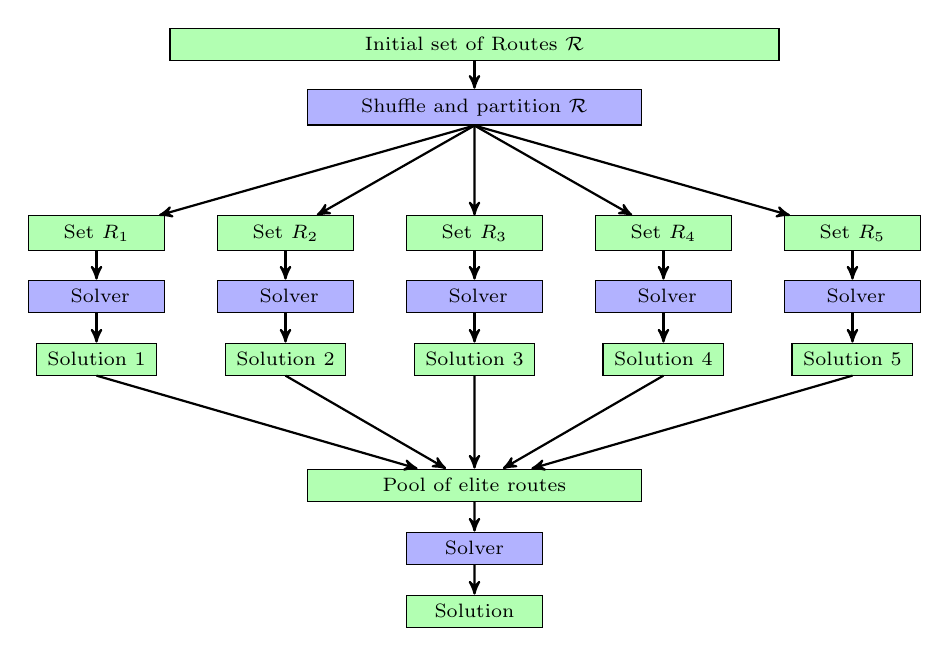
\begin{tikzpicture}[scale=0.8, auto,swap]
	
	\tikzstyle{instruct}=[rectangle, text width = 7.5cm, text  badly centered, draw]
	\tikzstyle{instruct2}=[rectangle, text width = 1.5cm, text  badly centered, draw,fill=green!30]
	\tikzstyle{instruct3}=[rectangle, text width = 1.5cm, text  badly centered, draw,fill=blue!30]
	\tikzstyle{instruct5}=[rectangle, text width = 1.3cm, text  badly centered, draw,fill=green!30]
	\tikzstyle{instruct4}=[rectangle, text width = 4cm, text  badly centered, draw]
	\tikzstyle{arc}=[->,>=stealth',thick,rounded corners=2pt, black]
	
	% placement des noeuds
	\node[instruct, fill=green!30] 	(s1) at (6,9) 	{\scriptsize{Initial set of Routes $\ro$}};
	\node[instruct4, fill=blue!30] 	(t1) at (6,8) 	{\scriptsize{Shuffle and partition $\ro$}};
	\draw[arc] (s1.south) -- (t1.north) ;
	\node[instruct2] 	(set1) at (0,6) 	{\scriptsize{Set $R_1$}};
	\node[instruct2] 	(set2) at (3,6) 	{\scriptsize{Set $R_2$}};
	\node[instruct2] 	(set3) at (6,6) 	{\scriptsize{Set $R_3$}};
	\node[instruct2] 	(set4) at (9,6) 	{\scriptsize{Set $R_4$}};
	\node[instruct2] 	(set5) at (12,6) 	{\scriptsize{Set $R_5$}};
	\draw[arc] (t1.south) -- (set1) ;
	\draw[arc] (t1.south) -- (set2) ;
	\draw[arc] (t1.south) -- (set3) ;
	\draw[arc] (t1.south) -- (set4) ;
	\draw[arc] (t1.south) -- (set5) ;
	\node[instruct3] 	(cplex1) at (0,5) 	{\scriptsize{ Solver}};
	\node[instruct3] 	(cplex2) at (3,5) 	{\scriptsize{ Solver}};
	\node[instruct3] 	(cplex3) at (6,5) 	{\scriptsize{ Solver}};
	\node[instruct3] 	(cplex4) at (9,5) 	{\scriptsize{ Solver}};
	\node[instruct3] 	(cplex5) at (12,5) {\scriptsize{ Solver}};
	\draw[arc] (set1.south) -- (cplex1.north) ;
	\draw[arc] (set2.south) -- (cplex2.north) ;
	\draw[arc] (set3.south) -- (cplex3.north) ;
	\draw[arc] (set4.south) -- (cplex4.north) ;
	\draw[arc] (set5.south) -- (cplex5.north) ;
	\node[instruct5] 	(sol1) at (0,4) 	{\scriptsize{Solution $1$}};
	\node[instruct5] 	(sol2) at (3,4) 	{\scriptsize{Solution $2$}};
	\node[instruct5] 	(sol3) at (6,4) 	{\scriptsize{Solution $3$}};
	\node[instruct5] 	(sol4) at (9,4) 	{\scriptsize{Solution $4$}};
	\node[instruct5] 	(sol5) at (12,4) 	{\scriptsize{Solution $5$}};
	\draw[arc] (cplex1.south) -- (sol1.north) ;
	\draw[arc] (cplex2.south) -- (sol2.north) ;
	\draw[arc] (cplex3.south) -- (sol3.north) ;
	\draw[arc] (cplex4.south) -- (sol4.north) ;
	\draw[arc] (cplex5.south) -- (sol5.north) ;
	\node[instruct4, ,fill=green!30] (pool) at (6,2) 	{\scriptsize{Pool of elite routes}};
	\draw[arc] (sol1.south) -- (pool) ;
	\draw[arc] (sol2.south) -- (pool) ;
	\draw[arc] (sol3.south) -- (pool) ;
	\draw[arc] (sol4.south) -- (pool) ;
	\draw[arc] (sol5.south) -- (pool) ;
	\node[instruct3] 	(cplex) at (6,1) 	{\scriptsize{Solver}};
	\draw[arc] (pool.south) -- (cplex) ;
	\node[instruct2]		(end)	at (6,0) {\scriptsize{Solution}};
	\draw[arc] (cplex.south) -- (end) ;
	
	\end{tikzpicture}
	\caption{Simplified scheme of the sampling heuristics}
	\label{fig:algo1}
\end{figure}

Figure \ref{fig:algo1} presents an idealistic situation in which 
(i) the quality of the solution is not too sensitive to the initial decomposition  into subsets $R_i$  
(ii) each subset $R_i, i \in 1\dots, \alpha$ yields a feasible instance that can be solved to optimality in reasonable computing time
(iii) the pool of elite routes also yields a feasible instance tractable with the MILP solver. 

The general principle described in \ref{fig:algo1} must be reinforced in order to manage the capacity of the MILP solver to solve subproblems and exhibit a good pool of elite routes. 


\subsection{Main scheme of the RSH algorithm} \label{sec:RSH}


Algorithm \ref{mainalgo} gives a more detailed description of our implementation of the RSH algorithm. 
Several iterations of the process described by Figure 1 are necessary, in order to iteratively refine the elite pool through distinct successive decompositions of the set $\ro$. 
 

\begin{algorithm}
	\caption{The Route Sampling Heuristic}
	\label{mainalgo}
	%\scriptsize
	\begin{algorithmic}[1]
		\REQUIRE  The set $\ro$ of all routes generated
		\REQUIRE A parameter $\alpha$ (number of subsets)
		\REQUIRE $t_1, t_2$: CPU (time budget) allocated to the MILP solver
		\REQUIRE $MaxIter$ : parameter
		\STATE $z^*= +\infty$
		\STATE $eliteRoutes \leftarrow \emptyset$
		\REPEAT
		\STATE $improve = FALSE$
		\STATE $\ro =  \ro \backslash eliteRoutes$
		\STATE Shuffle routes in $\ro$
		\STATE $LocationSampling(R,\alpha)$ \COMMENT{partitions $\ro$ into at most $\alpha$ subset of routes, regrouped by starting DC}
		\STATE $RouteSampling(R,\alpha)$	\COMMENT{partition $\ro$ into $\alpha$ independent subsets of routes}
		\FOR{$s=1$ to $\alpha$}
		\STATE $R_s = $ routes in subset $s$
		\STATE $bestRoutes_s = \emptyset$
		\FOR {$i=1$ to $MaxIter$}
		\STATE $(z,bestRoutes_s) = solveLIRP(R_s,t_1)$ 
		\STATE $eliteRoutes \leftarrow eliteRoutes \cup bestRoutes_s$
		\STATE $R_s \leftarrow R_s \backslash bestRoutes_s$
		
		\ENDFOR
		\ENDFOR
		\STATE 	$(z,bestRoutes) = solveLIRP(eliteRoute, t_2)$
		\IF {$z < z^*$}
		\STATE $z^*=z$
		\STATE $improve =TRUE$
		\ENDIF
		\UNTIL {$improve = FALSE$}
		\RETURN $bestRoutes$
	\end{algorithmic}
\end{algorithm}


The RSH algorithm is initialized with the set of routes and several parameters that control the number of subsets as well as time budget values ($t_1$ and $t_2$) allocated to the solver. 
The main loop (lines 3--23) repeats as long as the objective function is being improved. 
Each loop consists of running the algorithm represented by Figure \ref{fig:algo1}. 
Elite routes found at one given iteration are not considered anymore during subsequent iterations (line 5). This help find new elite routes and, thus, favors diversification. 


 generating of partition of the set of routes into subsets, solving each subset independently and collecting  (line 13) and collecting elite routes (line 14)

In lines 12-16, sets $R_1$--$R_\alpha$ can be repeatedly used to progressively exhibit new elite routes. 
If parameter $MaxIter$ is set at value 1, the situation is like that presented by Figure \ref{fig:algo1}. 
It $MaxIter > 1$,  all routes belonging to the solutions returned by the MILP solvers are saved in the pool of elite routes and removed from the current subsets $R_1 - R_\alpha $. 
In total, the MILP solver is called $MaxIter$ times, giving more opportunity to enrich the pool of elite routes. 

\subsection{Detail of the key procedures} \label{sec:details}


\paragraph{LP-rounding pre-processing}

	The idea of LP-rounding is to solve the linear relaxation of some MILPs, 
	and to round variables with fractional value to recover integer feasible solutions. 
	Despite its poor formal guarantee of performance, LP-rounding is known to yield good lower bounds 
	for some optimization problems including assignment problems ((\cite{BvN82}), \cite{FW07}), 
	lot-sizing problems (\cite{HNS07}), facility location (\cite{LSS2012}, \cite{CPS06}), 
	and supply chain network design problems  (\cite{VMN06}, \cite{Thanh2010}).
	
	In the preprocessing step of the RSH algorithm, we solve the linear relaxation of the LIRP model. All routes which corresponding variable $z_{rt}$ has a fractional value larger than or equal to a given parameter $\bar{z}$ \OP{notation a modifier?} are directly placed in the elite pool and removed from set $\ro$.
	
	
\paragraph{Case of direct routes}

	Consider one subset $R_i$ obtained from the decomposition of $\ro$ and the corresponding LIRP subproblem. it may happen that no route in $R_i$, or only ``bad routes'' visit some locations. To avoid the risk of unfeasibility and to help the MILP solver to find good solutions, direct routes from the origin(s) to the destinations of the routes are added to each subset $R_i$. 
	


\paragraph {Termination criteria}

\OP{Stop when the number of routes in the pool is large enough? 
	criteria based on CPU time? on improvement of the current solution? }

\OP{Preciser articulation entre locatio based sampling (ligne 7) et route sampling (ligne 8) }

\subsection{Location based sampling}


\paragraph{Model associated with one DC}

In this section, we present a DC-based decomposition that is used in ``direct-loop'' networks such as the one described by Figure \ref{fig:dl}. 
For each potential DC location $\lambda\in \loc_1$, we define a subproblem $P_{\lambda}$ with the following 
two types of routes: 
a unique route $r_0$ from the supplier to DC
and the set $\ro_2(\lambda)$ of routes at level 2 starting from DC $\lambda$, where 
$\ro_2(\lambda)=\left\{r\in\ro_2: \beta_{\lambda r}=1\right\}$ 
%
%Moreover, we define $\ro(\lambda)= \ro_1(\lambda) \cup \ro_2(\lambda)$. 

The set of clients is restricted to $\cu(\lambda) =\{i\in\cu: \sum_{r\in\ro_2(\lambda)} \alpha_{ir}\geq 1 \}$, i.e. clients that are reachable by at least a route starting from DC $\lambda$. 
Hence problem $P_{\lambda}$ is an inventory routing problem derived from the original LIRP, in which location decisions as well as routing decisions at level 1 have been discarded. 
Variables of the original MILP remain the same. 
The following MILP is a valid formulation of $P_{\lambda}$:
%
\begin{alignat}{3}
	\text{min} &&\sum_{t=1}^{T} \left( \sum_{r\in \{r_0\} \cup \ro(\lambda)} c_r z_{rt} + \sum_{i\in \left\{\lambda\right\}\cup \cu(\lambda)} h_{it} I_{it}\right) \span\omit\label{decomp_objfunct}\\ 
	\text{s.t.}  %&&\sum_{r\in \ro} \gamma_{jr} z_{rt} &\leq 1 															&\forall j&\in \, \forall t=1,\ldots,T  \label{const:singleroutedepots}\\
	&&\sum_{r\in \ro_2(\lambda)} \alpha_{ir} z_{rt} &\leq 1 															&\forall i&\in \cu(\lambda), \forall t\in T  \label{const:decomp_singleroutecustomers}\\
	&&\sum_{r\in \ro_2(\lambda)} z_{rt} &\leq 	\nu_2		&\forall t&\in T  \label{const:decomp_fleetcapa}\\
	%          &&\sum_{r\in \roc} z_{rt} &\leq 	\nu_{\cu}						&\forall t&=1,\ldots,T  \label{const:fleetcapaclients}\\
	&&x_{\lambda r_0 t}   		&\leq Q_1 z_{rt} 		&\forall t&\in T\label{const:decomp_deliveryDCUB}\\
	&&\sum_{i\in \cu(\lambda)} x_{irt}   		&\leq Q_2 z_{rt} 														&\forall r&\in \ro_2(\lambda), t\in T\label{const:decomp_deliveryUB}\\
	&&x_{irt}   		&\leq \alpha_{ir} Q_2  			&\forall i&\in\cu(\lambda), \forall r\in \ro_2(\lambda), t\in T\label{const:decomp_deliveryConstLoc}\\
	&&I_{\lambda t}- I_{\lambda,t-1} &=     x_{\lambda r_0 t}   - \sum_{r\in \ro_2(\lambda)}\left( \sum_{i\in \cu(\lambda)}x_{irt}\right)\quad 			&\forall t& \in T \label{const:decomp_invflowdepots}\\
	&&I_{it} - I_{i,t-1} &= \sum_{r\in \ro_2(\lambda)} x_{irt} - d_{it} 			&\forall i&\in \cu(\lambda), \forall t\in T\label{const:decomp_dinvflowcustomers}\\
	&&I_{\lambda t}	&\leq I_\lambda^{\max}  			& \forall t&\in T\label{const:decomp_invdepotUB}\\	
	&&I_{it} 		& \leq \min\left(I_i^{\max}, \sum_{t' > t}d_{it'}\right)											&\forall i&\in \cu(\lambda), \forall t\in T\label{const:decomp_invcustUB}\\
	&&x_{irt}			&\geq 0 							&\forall i&\in \cu(\lambda), \forall r\in \ro_2(\lambda),\forall t \in T\label{const:decomp_qpos}	\\
	&&x_{\lambda r_0 t}			&\geq 0 				&\forall t&\in T\label{const:decomp_qdcpos}	\\
	&&I_{it}	&\geq 0 			&\forall i &\in \{\lambda\}\cup \cu(\lambda), \forall t\in T\label{const:decomp_invCpos}	\\
	&&z_{rt}		&\in \{0,1\} 	&\forall r&\in \ro_2(\lambda), \forall t\in T\label{const:decomp_zbool}
\end{alignat}


Location based sampling is performed in two steps.
First, the clients are pre-assigned to a number of DCs, as described in Algorithm \ref{algo:pre-allocation}.
Then, this pre-assignment is used to build location-based subsets of routes, as described in Algorithm \ref{algo:location-sampling}.

\subsubsection{Pre-allocation of clients to DCs}

One important issue in supply chain network design is the allocation of customer to DCs. 
Constraint ~\eqref{const:singleroutecustomers} states that customers are delivered by at most one route everyday. 
Since we don't impose single-sourcing constraints, customers can be served by different DCs at distinct periods. 
So far, not all allocations of customers to DCs make sense. 

Algorithm \ref{algo:pre-allocation} is used to pre-allocate clients to a non-empty subset of relevant DCs. 
%
\begin{algorithm}
	\caption{Pre-allocations of clients to DCs}
	\label{algo:pre-allocation}
	%\scriptsize
	\begin{algorithmic}[1]
		\REQUIRE  $\loc_1$: set of DCs, $\cu$: set of clients, $N_{close}, \mu_1, \mu_2, \mu_3$: parameters, 
		$dist$: $|\cu|\times (|\loc_1|+|\cu|)$ distance matrix between clients and other clients + DC
		\STATE Initialization: $A$: $|\cu| \times |\loc_1|$ pre-allocation matrix filled with zeros
		\FOR {all clients $i \in \cu$}
		\STATE $ClosestDepots(i) = $ List of all DCs $j \in \loc_1$ ranked in non-decreasing order of the distances $dist(i,j)$.
		\STATE 	$A(i,ClosestDepots(i)[1]) =1$ 	
		\FOR {$n=2$ to $N_{close}$}
		\IF {$dist(i,ClosestDepots(i)[n]) < \mu_1$}
		\STATE 	$A(i,ClosestDepots(i)[n]) =1$ 			
		\ENDIF
		\ENDFOR
		\ENDFOR
		\FOR {all clients $i \in \cu$ }
		\STATE Rank clients $i' \in \cu$, $i' \neq i$ in non-decreasing order of the distances $dist(i,i')$ 
		\FOR {all clients $i'$ such that $dist(i,i') < \mu_2$} 
		\FOR {all $j \in ClosestDepots(i')$ such that $A(i',j)=1$}
		\IF {$A(i,j)=0$ and $dist(j,i)+dist(i,i')+dist(i',j) < \mu_3$}
		\STATE $A(i,j) =1$
		\ENDIF
		\ENDFOR
		\ENDFOR
		\ENDFOR
		\RETURN $A$
	\end{algorithmic}
\end{algorithm}
%
This pre-allocation algorithm returns a $|\cu| \times |\loc_1|$ matrix that defines a list of potential allocations for each client. 
The main loop (line 2-10) fills the pre-allocation matric for each client $i \in \cu$. 
Given a client $i$, all DCs $j \in \loc_1$ are ranked in non-decreasing order of their distance to $i$. 
First, $i$ is pre-allocated to its closest DC without any distance condition (line 4). 
Then, $i$ is allocated to its $N_{close}$ nearest DCs provided they lie at a distance not larger than a given value $\mu_1$ (line 5-8).

The second loop (lines 11--20) implements a pre-allocation rule that relaxes the distance constraint imposed by $\mu_1$ 
in the presence of clusters of clients. 
Let us consider two neighborhing clients $i_1$ and $i_2$, pre-allocated to DCs $j_1$ and $j_2$ respectively,
 as represented in Figure \ref{fig:prealloc}, 
Assuming that $dist(i_1,j_2) > \mu_1$, $i_1$ will be allocated to $j_2$ provided 
$dist(j_2,i_1) + dist(i_1,i_2) + dist(i_2,j_2) < \mu_3$. 

 
 \begin{figure}[htbp]
 	\centering
 	\begin{tikzpicture}[scale=0.8, auto,swap]
 	
 	\tikzstyle{client}=[circle,  text  badly centered, draw, color=black]
 	\tikzstyle{depot}=[circle, text  badly centered, draw, color=red]
 	\tikzstyle{value}=[color=blue]
 	\tikzstyle{arc}=[->,thick, blue]
 	\tikzstyle{arc2}=[dotted, black]
 	
 	% placement des noeuds
 	\node[client] (c1) at (5,5) {$i_1$};
 	\node[client] (c2) at (5,6.5) {$i_2$};
 	\node[depot] (d1) at (3,3) {$j_1$};
 	\node[depot] (d2) at (8.5,6.5) {$j_2$};
 	
 	\draw[arc2] (d1) -- (c1) ;
 	\draw[arc2] (d2) -- (c1) ;
 	\draw[arc2] (d2) -- (c2) ;
 	\draw[arc] (c2) to [ bend left]   (d2)  ;
 	\draw[arc] (c1) to [ bend left] (c2) ;
 	\draw[arc] (d2) to [ bend left]  (c1) ;
 	\node[value] (mu3) at (6.5,7.5) {\scriptsize $route length \leq \mu_3$};
 	
 	\node[client] (o) at (12,5) {};	
 	\node[depot] (d) at (14,5) {};
 	\draw[arc2] (o) -- (d);
 	\node[] () at (16,5) {\scriptsize Pre-allocation};
 	\node[client] (o') at (12,4) {};	
 	\node[client] (d') at (14,4) {};
 	\draw[arc] (o') -- (d');
 	\node[] () at (16,4) {\scriptsize Route arc};
 	
 	
 	\end{tikzpicture}
 	\caption{Pre-allocation in clusters}
 	\label{fig:prealloc}
 \end{figure}
 






%------------------------------------------------------------

\newpage 
\subsubsection{Heuristic selection of DCs}

 This matrix will be later modified in Algorithm \ref{algo:location-sampling} once open DCs are selected. 


Algorithm \ref{algo:location-sampling} describes the selection of DCs based on the pre-allocation of clients to DCs defined by Algorithm \ref{algo:pre-allocation}. 

\begin{algorithm}
	\caption{Heuristic selection of DCs}
	\label{algo:location-sampling}
	%\scriptsize
	\begin{algorithmic}[1]
		\REQUIRE $\loc_1$: set of DCs, $\cu$: set of clients, $A$: pre-allocation matrix, $p$: number of DCs to be selected, $\gamma>1$: parameter.
		\STATE  $A' \leftarrow$  $|\cu| \times |\loc_1|$ allocation matrix filled with zeros
		\STATE $S \leftarrow \emptyset$: list of selected DCs
		\STATE $n \leftarrow 0$: number of clients assigned to some DC
		\WHILE {$|S| < p$ and $n < |\cu|$ } 
			\STATE $ \loc_1 \leftarrow \loc_1 \backslash S$
			\STATE Rank $\loc_1$ by non-increasing order of the number of clients pre-allocated to each DC by Algorithm 
\ref{algo:pre-allocation}
			\STATE Choose a random value $v$ in interval $[0,1)$]
			\STATE $j \leftarrow$ DC at position $\lceil v^\gamma \times |\loc_1| \; \rceil$ in $\loc_1$.
			\FOR {all clients $i \in \cu$}
				\IF {$A[i][j] =1$}
					\STATE $A'[i][j] = 1$
					\STATE $n \leftarrow n+1$
					\FOR {all DCs $j' \neq j$}
						\STATE $A[i][j'] = 0$ 
					\ENDFOR
				\ENDIF		
			\ENDFOR
		\ENDWHILE
		\IF {$n < |\cu|$}
			\STATE Add a dummy DC $\delta$
			\FOR {all $i\in \cu$ such that $\sum\limits_{j \in \loc_1} A[i][j] >0$}
				\STATE $A'[i][\delta]=1$
			\ENDFOR
		\ENDIF
		\RETURN $S$ and $A'$
	\end{algorithmic}
\end{algorithm}

All non selected DC are ranked by non-increasing number of clients pre-allocated to them (line 6).
Then, a DC randomly is selected using a biased roulette wheel selection mechanism giving a much higher probability to the first DCs (lines 7--8). 
Since Algorithm \ref{algo:location-sampling} is called repeatedly in Algorithm \ref{mainalgo}, this randomized selection favours diversification. 

After selecting a DC, all clients that were pre-allocated to this DC are now allocated to it (lines 10--11) 
and their pre-allocation to all other DCs is cancelled (line 14). 
The final loop (lines 19--24) is used to allocate remaining clients to a dummy DC. 

\textcolor{red}{Olivier: Là je ne suis plus très sûr. Pourquoi est-ce important d'allouer les clients restant à un dépot ? Que fait-on si on n'a pas sélectionné $p$ dépots ? Et d'ailleurs comment la valeur de $p$ est elle choisie ? }

\textcolor{red}{Olivier: Question: can we have a selected DC with no customer allocated to it? If yes, remove these DCs}


\newpage

\subsubsection{Filtering SD routes after DC selection}

After selecting a subset of DCs and allocating clients to selected DCs, routes must be filtered in order to remove useless ones. 
In the first $L-1$ levels, all routes that contain at least one unselected DC are removed from the route set. 
In the last level, routes that start at unselected DCs are removed from the route set, as well as routes visiting clients that are not allocating to the starting DC. 



\section{Strengthening the formulation}
\subsection{A difference approach}
\begin{table}[htbp]
\centering
\begin{tabular}{ll}
\toprule
$f_j$ & Fixed cost of opening distribution center $j\in\loc \setminus \cu$\\ 
$d_{it}$ & Demand of customer $i\in\cu$ in period $t \in T$\\
        $h_{it}$ & Unitary holding cost at facility $i\in\loc$ in period $t \in T$\\
        $c_r$ & Cost of route $r\in \ro$\\
        $\alpha(r)$ & Set of facilities $i$ delivered by route $r$\\
        $\beta(r)$ & Index of the starting DC of route $r$\\
        $Q_k$ & Capacity of vehicles delivering locations at level $k$\\ 
        $\nu_k$ & Fleet size for vehicles delivering locations of level $k$\\ 
        \bottomrule
        \end{tabular}
        \caption{Data}
        \label{tab:data}
        \end{table}       
        \begin{table}[htbp]
        \centering
        \begin{tabular}{ll}
        \toprule
        \multicolumn{2}{l}{\textit{Binary Variables}}\\
            $y_{j}$ & $=1$ if distribution center $j \in \loc \backslash \cu$ is selected \\
            $z_{rt}$ & $=1$ if route $r \in \ro$  is selected in period $t \in T$\\
            \midrule
            \multicolumn{2}{l}{\textit{Continuous variables}}\\
                $x^{it}_{js}\in[0,1]$ & Proportion of demand $(i,t)$ delivered to location $j\in \loc$ in period $s\leq t$\\
                \bottomrule
                \end{tabular}
                \caption{Variables}
                \label{tab:var}
                \end{table}    

                %Partition the demand points in time and space. Accessible demand points are on a given route starting from a given source, and only the future periods are considered.
                \begin{alignat}{3}
                    \text{minimize} &&\sum_{j\in \loc \setminus \cu} f_{j} y_{j} +\sum_{t=1}^{T} \left( \sum_{r\in \ro} c_r z_{rt} + \sum_{i\in \cu} \sum_{j\in\loc}\sum_{s=1}^t h^{it}_{js}x^{it}_{js}\right)\span\span\label{objfunct2}\\ 
    \text{s.t.}  %&&\sum_{r\in \ro} \gamma_{jr} z_{rt} &\leq 1 															&\forall j&\in \, \forall t=1,\ldots,T  \label{const:singleroutedepots}\\
    &&\sum_{r : i\in\alpha(r)} z_{rs} &\leq 1 															&\forall i&\in \loc, \forall s=1,\ldots,T  \label{const:singleroutecustomers2}\\
    &&\sum_{r : j\in\alpha(r)} z_{rs} &\leq y_j 															&\forall j&\in \loc\setminus \cu, \forall s=1,\ldots,T  \label{const:singleroutedc2}\\
    %&&\gamma_{jr}z_{rt} 					&\leq y_j 													&\forall k&=1,\ldots,L, \forall j\in\loc_{k-1}, \forall r\in \ro_k, \forall t=1,\ldots,T\label{const:serveopendepots}\\
    &&z_{rs} 					&\leq y_{\beta(r)} 													&\forall r&\in \ro, \forall s=1,\ldots,T\label{const:startfromopendepots2}\\
    &&\sum_{r\in \ro_k} z_{rs} &\leq 	\nu_k													&\forall k&=1,\ldots,L, \forall s=1,\ldots,T  \label{const:fleetcapa2}\\
    %            &&\sum_{r\in \roc} z_{rt} &\leq 	\nu_{\cu}													&\forall t&=1,\ldots,T  \label{const:fleetcapaclients}\\
    &&\sum_{s=1}^t x^{it}_{is}   		& = 1 														&\forall i&\in \cu, \forall t=1,\ldots, T\label{const:satdemands}\\
    &&x^{it}_{js}   		&\leq \sum_{r\in\ro : j\in\alpha(r)} z_{rs}													&\forall i&\in \cu, t=1,\ldots,T, s=1,\ldots,t,j\in\loc\setminus\cu\cup\{i\}\label{const:deliveryConstLoc2}\\
    &&\sum_{i\in\cu}\sum_{t=s}^T\sum_{j\in\alpha(r)} d_{it} x^{it}_{js}   		&\leq Q_k z_{rs} 														&\forall k&=1,\ldots,L, \forall r\in \ro, s=1,\ldots,T\label{const:deliveryUB2}\\
    %&&\sum_{i\in \cu} u^t_{ir}   		&\leq \kc z_{rt} 														&\forall r&\in \roc, t=1,\ldots,T\label{const:deliveryUBcustomers}\\
    &&\sum_{u=1}^s \left(\sum_{j\in\loc_{k}} x^{it}_{js} - \sum_{l\in\loc_{k+1}} x^{it}_{ls}\right) &\geq 0\quad 			&\forall k&=1,\ldots,L-1, \forall i\in\cu, \forall t=1,\ldots,T \label{const:enoughunits}\\
 %   &&I_{jt}					&\leq I_j^{\max} y_j  									&\forall k&=1,\ldots,L-1, \forall j\in \loc_k,\forall t=1,\ldots,T\label{const:invdepotUB2}\\	
 %   &&I_{it} 					&\leq \min\left(I_i^{\max}, \sum_{t' > t}d_{it'}\right)											&\forall i&\in \cu, \forall t=1,\ldots,T\label{const:invcustUB2}\\
    &&x^{it}_{js}			&\geq 0 															&\forall i&\in \cu,\forall t=1,\ldots, T, \forall j\in \loc\setminus\cu\cup\{i\}, \forall s= 1,\ldots t\label{const:upos2}	\\
    &&y_{j}					& \in \{0,1\} 														&\forall j&\in \loc\setminus\cu\label{const:ybool2}\\	
    &&z_{rs}					&\in \{0,1\} 														&\forall r&\in \ro, \forall s=1,\ldots,T\label{const:zbool2}
\end{alignat}

Constraint~\eqref{const:singleroutecustomers2} ensures that a customer is served by at most one route in each period.
Constraint~\eqref{const:singleroutedc2} ensures that a dc is served by at most one route in each period.
Constraint~\eqref{const:startfromopendepots2} ensures that each active route in period $s$ start from an open dc.
Constraint~\eqref{const:fleetcapa2} ensures that there are no more active routes than the number of vehicles in period $s$.
Constraint~\eqref{const:satdemands} ensures that all demands are satisfied.
Constraint~\eqref{const:deliveryConstLoc2} ensures that units can be delivered to location $j$ in period $s$ only if it belongs to an active route in this period.
Constraint~\eqref{const:deliveryUB2} ensures that a vehicle using a route $r$ in period $s$ do not deliver more units than its capacity.
Constraint~\eqref{const:enoughunits} ensures that units delivered to the locations in a given layer are present on the upper level of the network.


%--------------------------
\section{Numerical experiments}
\label{sec:expe}
\subsection{Generation of instances}

\paragraph{Assumptions}
\begin{itemize}
    \item The cost of transportation is proportional to the duration of the route
    \item The speed of the vehicles is equal to 45 km/h.
    \item The capacity of the vehicles is fixed
    \item Demand vary from one period to the next and from one client to another, as {\em high}, {\em low} or {\em mixed}
    \end{itemize}


\paragraph{Generation of routes}

\OP{Paragraph a rédiger}

Considering one starting DC and $n$ customers, the number of potential routes visiting at most $m$ customers 
is $\mathcal{O}(n^m)$.

In practice, \textbf{long-haul carriers} are reluctant to perform routes with multiple stop and with long detours between the origin and the destination of their routes. 

\begin{itemize}
	\item stopover cost
	\item max detour constraint
\end{itemize}
This limit the set of potential routes. 

Add references \OP{chercher les bonnes réfs dans thèse Juliette}

Last-mile deliveries / messagerie : routes with regular activities with frequent deliveries (postal services): many customer on a route. This relies on the assumption that (i) customers must be served frequently and (ii) represent a small part of the total vehicle capacity. In this case, logistics operators define template routes with multiple customers. These routes are operated everyday ; the drivers just skip customers with no demand on a given day. 

If conditions (i) and (ii) are not satisfied: route cannot have multiple stops. Routes may change every day. 

Large regions covered by a DC are divided into geographical areas. It is frequently assumed that a given route visits only customers in a given area.


\cite{Zheng2019} restrict the number of variables by incorporating real-life constraints that are not part of their mathematical model: vehicles can visit at most four retailers at one trip due to vehicle capacity limitation, and DCs can only serve retailers within a given radius. These constraints help reduce the number of variables from 3 millions to 600 thousands.

Our assumption : route length is limited both in time (working time regulation), in the number of customers visited and in areas.   Each route has a maximum duration, including the stops and the travel durations



\paragraph{Methodology}
We obtain different instances of LIRP by positioning the different locations involved on a shared map, combining different {\em layers}, where each layer contains specific elements of the final problem.
carrying some of the elements of the final problem.
E
Specifically, we use the following procedure to build and combine the different layers:
\begin{description}
    \item[Urban areas] We start by positioning
    \item[Clients]
    \item[DCs]
    \item[Demand boxes]
\end{description}



\section{Conclusion}

\paragraph{Extension to multi-level instances}

Why do we consider routes at one level only? 

\begin{itemize}
	\item Distribution networks with multiple levels of routes: this requires combining routes obtained at each level. High combinatorial burden. 
	\item LIPR = hard problem. Probably not tractable with two many route levels. 
\end{itemize}





\subsection*{Possible extensions}
\begin{itemize}
	\item Load dependent route cost. 
	\item Generalisation to extended networks
	\item One warehouse multi retailer routing problem
	\item combination of collection and delivery activities
	
\end{itemize}


\end{linenumbers}

\newpage
%\bibliographystyle{abbrvnat}
\bibliographystyle{apalike}
\bibliography{biblio_LIRP}

\end{document}
